\documentclass{article}
\usepackage[utf8]{inputenc}
\usepackage{graphicx}

\title{Taller Hermite}
\author{Diego Barajas\\Brandonn Cruz}
\date{September 2018}

\begin{document}

\maketitle

\section{Problema}

Utilizar interpolación de hermite con la menor cantidad de puntos posibles para replicar de manera casi exacta el perfil del siguiente pato.

\begin{figure}[h!]
\centering
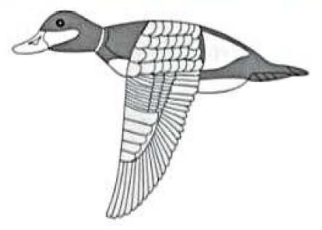
\includegraphics[scale=0.5]{pato.png}
\caption{Pato}
\label{fig:fisica}
\end{figure}

\section{Formalización}
\subsection{Entradas}

Valores X = [$x_0, x_1, ..., x_n$] y Y = [$y_0, y_1, ..., y_n$] tales que para cada pareja de datos $x_m$ y $y_m$ se pueden representar como f($x_m$) = $y_m$.

\subsection{Salidas}

Polinomio P(x) que permitan graficar el perfil del pato como se ve en la figura 2.

\begin{figure}[h!]
\centering
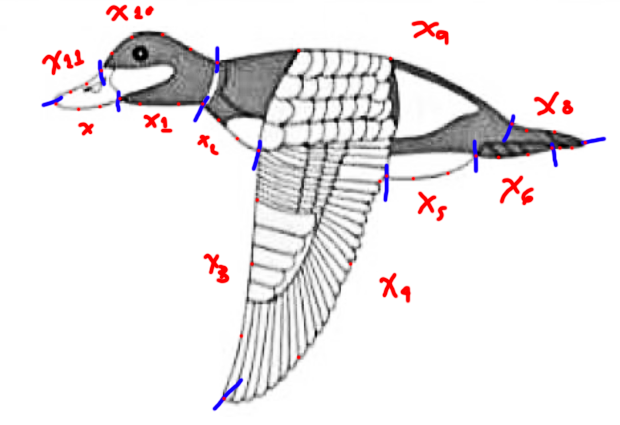
\includegraphics[scale=0.2]{pato2(1).png}
\caption{Dispersión de polinomios}
\label{fig:fisica}
\end{figure}

\newpage

\section{Implementación}
\\
\begin{equation} \label{Diferencias divididas}
f[x_0,...,x_n] = \frac{f[x_0,...,x_n_-_1]-f[x_1,...,x_n]}{x_0-x_n}
\end{equation}

\\
Para implementar el algoritmo de hermite recurrimos a utilizar la fórmula de Newton generalizada o también conocida como método de diferencias divididas.\\
El algoritmo implementado para el método de diferencias divididas consistes en realizar repetidas sumas y divisiones sobre los valores X y Y como se ve en la ecuacion 1 para encontrar un polinomio de la siguiente manera.


\begin{equation} \label{eu_eqn}
P_n(x) = A_0+A_1(x-x_0)+A_2(x-x_0)(x-x_1)+...+A_n(x-x_0)(x-x_1)...(x-x_n_-_1)
\end{equation}

Donde

\begin{equation} \label{eu_eqn}
A_0 = f[x_0]
\end{equation}

\begin{equation} \label{eu_eqn}
A_1 = f[x_0,x_1]
\end{equation}

\begin{equation} \label{eu_eqn}
A_n = f[x_0,x_1,...,x_n]
\end{equation}

\newpage

\section{Resultados}

Después de aplicar el algoritmo de hermite se generó la siguiente figura.

\begin{figure}[h!]
\centering
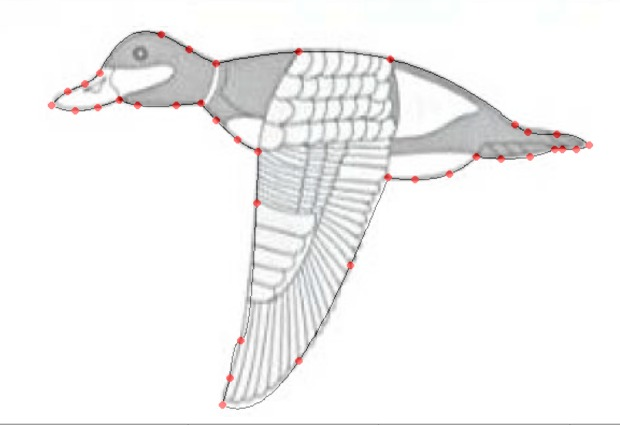
\includegraphics[scale=0.3]{pat.jpg}
\caption{Comparacion resultados contra figura real}
\label{fig:fisica}
\end{figure}


\section{Manual de compilación}

Ejecutar el archivo hermite.r.

\end{document}
